\begin{tikzpicture}
\coordinate (A) at (0,0); \coordinate (B) at (2.5,0);
\coordinate (C) at (4.25,0); \coordinate (D) at (5.5,0);
\coordinate (E) at (6.75,0); \coordinate (F) at (8,0);
\coordinate (G) at (10,0); \coordinate (H) at (12,0);
\coordinate (Mid) at (6,3); \coordinate (PreA) at (-0.5, 0);
\coordinate (PostH) at (12.5,0); \coordinate (key) at (10,2);
\draw[black, thick] (PreA) -- (PostH); \draw[violet, thick] (A) -- (Mid) -- (H); \draw[violet, thick] (B) -- (Mid) -- (G); \draw[violet, thick] (C) -- (Mid) -- (F); \draw[violet, thick] (D) -- (Mid) -- (E);
\filldraw[black] (A) circle (2pt) node[below = 2.5] {$x_0$};
\filldraw[black] (B) circle (2pt) node[below = 1] {$x_1'$};
\filldraw[black] (C) circle (2pt) node[below = 7] {\dots};
\filldraw[black] (D) circle (2pt) node[below = 1] {$x_i' = 0$};
\filldraw[black] (E) circle (2pt) node[below = 7] {\dots};
\filldraw[black] (F) circle (2pt) node[below = 1] {$x_j' = 1$};
\filldraw[black] (G) circle (2pt) node[below = 7pt] {\dots };
\filldraw[black] (H) circle (2pt) node[below = 1] {$x_{n-2}'$};
\filldraw[black] (Mid) circle (2pt) node[above right] {$[[0,1]]_{\alpha(i+1),\alpha(j+1)}$};
\draw[black] (A) ++(0.75,0) arc[start angle=0,end angle=40,radius=0.5] node[midway, right] {$\alpha$};
\draw[black] (B) ++(-0.4,0) arc[start angle=180,end angle=50,radius=0.5] node[above left, yshift = 2] {$\pi - 2\alpha$};
\draw[black] (B) ++(0.6,0) arc[start angle=0,end angle=49,radius=0.5] node[right] {\phantom{s}$2\alpha$};
\draw[black] (Mid) ++(-2,-1) arc[start angle=195,end angle=262,radius=.5] node[midway, left, yshift = -1 pt] {$\alpha$};
\draw[black] (4.4,1.65) arc[start angle=190,end angle=280,radius=0.5] node[midway, left, yshift = -2 pt] {$\alpha$};
\draw[black] (4.98,1.23) arc[start angle=190,end angle=318,radius=0.4] node[midway, yshift = -5 pt] {$\alpha$};
\draw[black] (5.68,1.02) arc[start angle=200,end angle=343,radius=0.43] node[midway, yshift = -3.5 pt] {$\alpha$};
\draw[black] (6.5,1.04) arc[start angle=200,end angle=337,radius=0.45] node[xshift = -7 pt, yshift = -11 pt] {$\alpha$};
\draw[black] (7.34,1) arc[start angle=270,end angle=355,radius=0.6] node[midway, right, yshift = -3.2 pt, xshift = -1.5] {$\alpha$};
\draw[black] (7.95,1.54) arc[start angle=270,end angle=351,radius=0.35] node[midway, xshift = 5pt, yshift = -2 pt] {$\alpha$};
\node at (key) {$\alpha = \dfrac{\pi}{n}$};
\end{tikzpicture}